\documentclass[a4paper]{article}

%%%%%%%%%%%%%%%%%%%%%%%%%%%%%%%%%%%%%%%%%%%%%%
\usepackage[T1]{fontenc}
\usepackage{geometry}
\geometry{a4paper,left=1.5cm,right=1cm,top=1cm,bottom=1cm}

\usepackage{graphicx}
\usepackage[absolute,overlay]{textpos}
\usepackage{eso-pic}               % image de fond
\usepackage{fontawesome5}
\usepackage[hidelinks]{hyperref}
\usepackage{tikz}
\usepackage{xcolor}
\usepackage{enumitem}
\setlist{nosep,leftmargin=6mm}
\usepackage{times}                % même police que votre exemple
\usepackage{array} 
\usepackage{tabularx}
\usepackage{ragged2e}
\let\origcolorbox\colorbox    % sauvegarde
\renewcommand{\colorbox}[2]{#2}% neutralise le fond
%%%%%%%%%%%%%%%%%%%%%%%%%%%%%%%%%%%%%%%%%%%%%%
%\definecolor{texcolor}{HTML}{e2e8f0}
\providecolor{sidetext}{rgb}{1,1,1}
\definecolor{maincolor}{HTML}{ffffff}

%%%%%%%%%%%%%%%%%%%%%%%%%%%%%%%%%%%%%%%%%
% — Ne changez pas le nom : « background.jpg » doit être présent
\AddToShipoutPictureBG*{%
  
\includegraphics[width=\paperwidth,height=\paperheight]{background.jpg}%
}

%%%%%%%%%%%%%%%%%%%%%%%%%%%%%%%%%%%%%%%%%
\newcommand{\fullrule}{\hspace{-1.5cm}\rule{\paperwidth}{0.4pt}}
\newcommand{\cvsection}[1]{%
  \vspace{6pt}\textbf{\Large #1}\par\vspace{2pt}}
\newcommand{\cicon}[1]{%
  \tikz[baseline]{\draw[fill=white] (0,0.1) circle[radius=0.1cm];}~#1}

\setlength{\parindent}{0pt}
%\color{texcolor}
%%%%%%%%%%%%%%%%%%%%%%%%%%%%%%%%%%%%%%%%%%%%%%%%%%%%%%%%%%%%%%
\begin{document}
\color{white}
% ---------- Photo ------------------------------------------------
\begin{textblock*}{4cm}(0.2cm,0.3cm)
  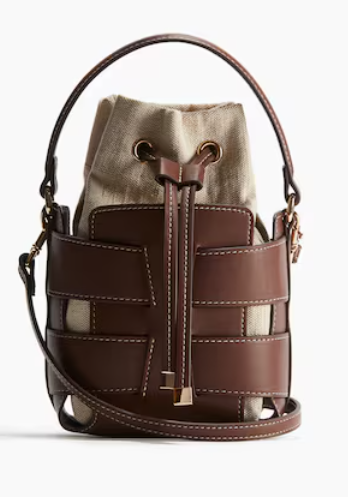
\includegraphics[width=2.5cm,clip,keepaspectratio]{94cad748eae3460791f872721fd4dca3.png}
\end{textblock*}

% ---------- En-tête ---------------------------------------------
\begin{center}
  {\fontsize{44pt}{24pt}\selectfont\bfseries Judikael Mourouvin}

  \bigskip
  {\Large Technicien informatique \& marketing digital}

  \bigskip\bigskip
  \faMapMarker~Route de Cocoyer\ 97190 Gosier
  \quad\faEnvelope~\href{mailto:jkmou971@gmail.com}{jkmou971@gmail.com}

  \bigskip
  % Badge LinkedIn (retirez-le si inutile)
  \faPhone~ +590 0690 91 14 48
  \quad \faLinkedin\ \href{}{}
 

  \vspace{-0.3cm}
  \fullrule
\end{center}

% ---------- Profil ----------------------------------------------
\cvsection{Profil}
\hspace*{2cm}%
Passionné d’informatique et de marketing digital, j’ai développé de solides compétences en configuration de postes, maintenance et résolution d’incidents. Mon année d’alternance à la DSI de la Mairie du Gosier m’a permis de gérer des projets numériques variés et d’accompagner les utilisateurs au quotidien. Rigoureux et réactif, je souhaite désormais mettre mon expertise technique et ma vision marketing au service de vos projets. Motivé et curieux, je m’investis pleinement pour garantir la réussite des missions confiées.

\medskip\fullrule

% ---------- Expérience ------------------------------------------
\cvsection{Expérience}
\hspace*{1.3cm}%

\colorbox{maincolor}{%
  \begin{minipage}{\linewidth}
    \textbf{Alternant en Marketing Digital} \\ Mairie du Gosier – DSI \\ 2023-2024
    \begin{itemize}
      \item Coordonné des projets numériques municipaux, assurant leur livraison conforme aux objectifs \item Analysé les besoins des agents et déployé des solutions adaptées, réduisant les demandes de support \item Dispensé un support technique et formé les utilisateurs, améliorant l’adoption des outils digitaux
    \end{itemize}
  \end{minipage}}

\vspace{3mm}


\colorbox{maincolor}{%
  \begin{minipage}{\linewidth}
    \textbf{Animateur de la zone informatique} \\ Pôle Emploi, Gosier \\ 2022-2023
    \begin{itemize}
      \item Assuré le support utilisateurs de la zone informatique, garantissant la continuité de service \item Configuré et maintenu les postes, réduisant les pannes récurrentes \item Diagnostiqué et résolu les incidents matériels et logiciels dans des délais courts
    \end{itemize}
  \end{minipage}}

\vspace{3mm}


\colorbox{maincolor}{%
  \begin{minipage}{\linewidth}
    \textbf{Stagiaire Informaticien} \\ Numerika, Baie Mahault \\ 2020-2021
    \begin{itemize}
      \item Configuré et entretenu le parc informatique, optimisant la performance des équipements \item Fournit un support de proximité aux collaborateurs, améliorant la satisfaction utilisateur
    \end{itemize}
  \end{minipage}}

\medskip\fullrule

% ---------- Éducation -------------------------------------------
\cvsection{Éducation}
\hspace*{1.3cm}%

    \begin{tabularx}{\linewidth}{@{}c >{\RaggedRight\arraybackslash}X@{}}
    \textcolor{sidetext}{\faGraduationCap} &
    \textbf{Bachelor Marketing Digital} \\
    & CFA IUTS \\
    & \textit{2023-2024} \\
    \end{tabularx}
    \begin{itemize}[leftmargin=*]
  \item Formation aux stratégies de marketing en ligne, SEO/SEA et réseaux sociaux
  \item Apprentissage de l’analyse de données et des KPI digitaux
  \item Gestion de projets de communication numérique
\end{itemize}
\vspace{3mm}

    \begin{tabularx}{\linewidth}{@{}c >{\RaggedRight\arraybackslash}X@{}}
    \textcolor{sidetext}{\faGraduationCap} &
    \textbf{BTS Systèmes Numériques option Informatique et Réseaux} \\
    & Lycée de Chevalier Saint Georges, Abymes \\
    & \textit{2019-2021} \\
    \end{tabularx}
    \begin{itemize}[leftmargin=*]
  \item Étude des architectures réseau et administration de systèmes
  \item Pratique de la maintenance matérielle et logicielle
  \item Mise en œuvre de projets d’intégration et de sécurisation IT
\end{itemize}

\medskip\fullrule

% ---------- Compétences -----------------------------------------
\cvsection{Compétences}

\hspace*{2cm}%
\begin{tabular}{@{}p{0.25\linewidth}p{0.18\linewidth}p{0.18\linewidth}p{0.18\linewidth}}\cicon Administration & \cicon Maintenance & \cicon Réseaux & \cicon Support \\
\cicon Assistance & \cicon Diagnostic & \cicon Marketing & \cicon Configuration \\
\cicon Analyse & \cicon Formation & ~ & ~ \\\end{tabular}   % grille 3 lignes × 4 colonnes

\end{document}
